\subsection{Background}
\subsubsection{Image Processing}
An image can be seen as a mathematical function $i(x,y)$ where $x$ and $y$ are the spatial coordinates and the output is a color at position $(x,y)$. If the color has a discrete quantities and the total image has a finite element of samples, it is called a \emph{Digital Image}. The samples each has a unique spatial coordinate and are referred to as \emph{pixels}. The field of \emph{Digital Image Processing} refers to processing a digital image and its pixels. Every time Image Processing is mentioned in this theis, it is assumed that it refers to Digital Image Processing. 
\newline

It is not obvious what 
\begin{figure}[ht!]
\centering

\includegraphics[width=80mm]{img/lena.png}
\caption{A blur algorithm is applied on an input image and produces a blurred output image.}
\label{lena}
\end{figure}

\begin{figure}[ht!]
\centering
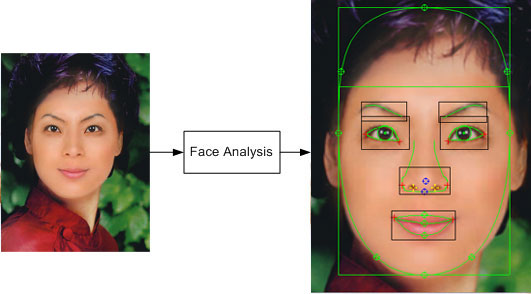
\includegraphics[width=80mm]{img/feature.jpg}
\caption{The input image of a face is analyzed to find features such as nose, mouth and eyes.}
\label{feature}
\end{figure}
